\section{Swarm intelligence}
\label{sec:swarmIntelligence}
Swarm behavior is found in many different species in nature, including fish schools and bird flocks. Many species practice swarm behavior for a biological need to stay together, because predators usually attack one individual, and not an entire flock. Swarm behavior is also found in social insects like ants, wasps, bees, and termites. They collaborate on tasks for building nests, gathering food and organizing production. These social insect colonies have demonstrated that simple organisms can perform complex tasks by continuously interacting with each other. The colonies are highly distributed and self-organized, and they adapt well to changes in the environment. Swarm intelligence (SI) \citep{beni89} is a branch of artificial intelligence that is strongly influenced by the swarm behavior found in the nature, attempting to adapt these characteristics in intelligent computer systems. SI based algorithms, such as the ones described in \ref{subsec:aco} - \ref{subsec:pso}, are metaheuristic optimization algorithms. Metaheuristic algorithms are typically used to find good solutions to combinatorial optimization problems, but they do not guarantee an optimal solution.  

\subsection{Ant colony optimization}
\label{subsec:aco}
In nature, ants have proven to be extremely capable of finding an optimal or close to optimal route from the nest to a food source \citep{deneubourg90}. Ants communicate by leaving a pheromone trail that other ants smell, and will follow by a certain probability. Most ant species leave a pheromone trail when returning to the nest from an important food source. The more pheromone units on a path (i.e. the more ants that have chosen it), the greater the probability that other ants will choose it. The pheromone units on a path found early, but later discarded in favor of a better path, will evaporate. This results in a smaller probability to be selected, and thus ensures that better routes are favored.

In nature, ants are adaptable to changes, and manage to find the shortest path even though an obstacle is added to the current shortest path. This is illustrated in Figure \ref{fig:ants}. To the left, the ants have found an efficient route. In the middle, an obstacle is added, and the ants explore different paths. To the right the ants have found the most efficient route around the obstacle.

\begin{figure}[H]
  \centering
  \includegraphics[width=3in]{assets/maur.png}
  \caption{An illustration of how ants adapt to change} 
   \label{fig:ants}
\end{figure}

Ant colony optimization (ACO) is a class of graph representation based algorithms designed to optimize routing problems. The first description of an ACO algorithm, called Ant System (AS), was initially proposed by \citet{dorigo96}. The AS strategy developed by Dorigo tries to simulate the behavior of real ants, but unlike the ants in nature, pheromone trails are left by all ants. Algorithm \ref{algo:aco} shows the metaheuristic of ACO, as described by \citet{dorigo06}:
\begin{algorithm}[H]
\caption{The Ant Colony Optimization Metaheuristic}
\label{algo:aco}
\begin{algorithmic}
\\ Set parameters, initialize pheromone trails
  \While{termination condition not met}
    \State ConstructAntSolutions
    \State ApplyLocalSearch (optional)
    \State UpdatePheromones
  \EndWhile
\end{algorithmic}
\end{algorithm}
~\\

The idea of ACO algorithms is to create a decentralized system with multiple artificial ants. The artificial ants, like the one found in nature, influence each others decisions by using ``pheromone''. In the beginning, before any distinct pheromone trail is laid, the artificial ants' choices are random, and thus they perform a broad search in the environment. This randomness will decrease over time as the pheromone trails become more distinct. At the end of each iteration an amount of the pheromone evaporates. This reduces the probability of the artificial ants getting stuck at local optima. 

Many versions of ACO algorithms have been proposed in the literature, and among the most successful are the Ant Colony System (ACS) proposed by \citet{dorigo97} and the MAX-MIN Ant System (MMAS) proposed by \citet{stutzle06}. The ACS implements both a \textit{local} and a \textit{global} pheromone update. The local pheromone update are applied by all artificial ants after each construction step, and the global pheromone update are applied by the evaluated best artificial ant at the end of each iteration. The MMAS only allows the evaluated best artificial ant to update the pheromone trail. The amount of pheromone given to the best path is determined, within a certain bound, by the quality of the solution found. 

\subsection{Bee colony optimization}
\label{subsec:BCO}
As described in \citet{lucic03}, bees are capable of performing a variety of complex tasks. Examples of these tasks are the collection and processing of nectar, which may be considered as very organized. The idea is that a bee that leaves the hive to gather nectar flies to the hives so-called ``dance floor''. The bees that already have found a good food source performs a ``dance'' at the dance floor to advertise that they have found a satisfying food source. Newly arriving bees will choose one of the dancers and follow it to the discovered food source. As stated in \citet{lucic03}, the mechanism of deciding which bee to follow is not well understood.  Nevertheless, it is considered that ``the recruitment among bees is always a function of the quality of the food source''. After a bee has gathered and returned the food to the hive, the bee has three options \citep{lucic03}:

\begin{enumerate}
  \item Abandon the food source and return to the dance floor, and again follow a dancing bee
  \item Continue to gather nectar from the food source without recruiting nest mates
  \item Return to the dance floor and dance, and thus recruit nest mates before returning to the food source
\end{enumerate}

Bee colony optimization (BCO) is a method that, like ACO, aims to create a decentralized optimization system with multiple agents, based on graph representation. The idea is to apply the collective intelligence of the food gathering process to an optimization system. Like a typical ACO algorithm, a typical BCO algorithm is inspired by the way bees acts in nature, but where some features are added, and some are removed. \citet{nikolic14} describes a BCO algorithm where the artificial bee only has two options after returning from a food source: (1) abandon or (2) recruit. \citet{lucic03} gives the artificial bees attributes such as memory and perfect knowledge about the quantity of nectar collected by other artificial bees. These modifications are done in order to be more suitable for performing complex combinatorial problems.

\subsection{Particle swarm optimization}
\label{subsec:pso}
As reported in \citet{shi99}, Particle Swarm Optimization (PSO) was first introduced by Eberhart and Kennedy in 1995. PSO is inspired by how the social behavior of flocks (such as flocks of birds) and schools (such as fish schools) cooperates. The idea is to update the individuals velocity according to the individual's experience and its companions' experience. This differs from other evolutionary computational algorithms, like Genetic algorithms, which uses evolutionary operators to manipulate the individuals. The basic concept is that each individual moves with a certain velocity and that this velocity is dynamically adjusted based on the experience. Each individual is a volume less particle (i.e. a point) in the D-dimensional search space. The \textit{i}th particle position is represented as $X_i = (X_{i1},X_{i2}...X_{iD})$. Each particle knows its own best position so far\footnote{The position that gave the highest fitness value}, represented as $P_i = (P_{i1},P_{i2}...P_{iD})$, and the best position \textit{g}, achieved among all the particles. These two positions are used to calculate the velocity, $V_i = (V_{i1},V_{i2}...V_{iD})$ ,  of the \textit{i}th particle \citep{shi99}: 

$$V_{id} = w * V_{id} + c_1 * rand() * (P_{id}-X_{id}) + c_2 * Rand() * (P_{gd}-X_{id})$$

where \textit{w} is a decreasing parameter called inertia weight added to PSO to balance local and global search, $c_1$ and $c_2$ are two positive constants, and \textit{rand()} and \textit{Rand()} are two random functions in the range [0,1]. Figure \ref{fig:psoBeginning} illustrates how the particles in PSO explore in the early iterations of the algorithm, while figure \ref{fig:psoEnd} illustrates how the particles tend to act more organized and coordinated at the late iterations. The new position of the \textit{i}th particle is calculated as follows \citep{shi99}:

$$X_i = X_{id} + V_{id}$$

Because of the decreasing inertia weight, PSO may suffer from low global search ability at the end of the run, and thus risking getting stuck at a local optimum. This may result in the algorithm failing to find the required optimum when the problem to be solved is very complicated and complex \citep{shi99}. However, PSO has proven to create sufficient solutions to NP-hard problems including the Multi-Dimensional Knapsack Problem \citep{wan09} and the Urban Transit Routing Problem \citep{kechagiopoulos14}. 

\begin{figure}[H]
  \centering
  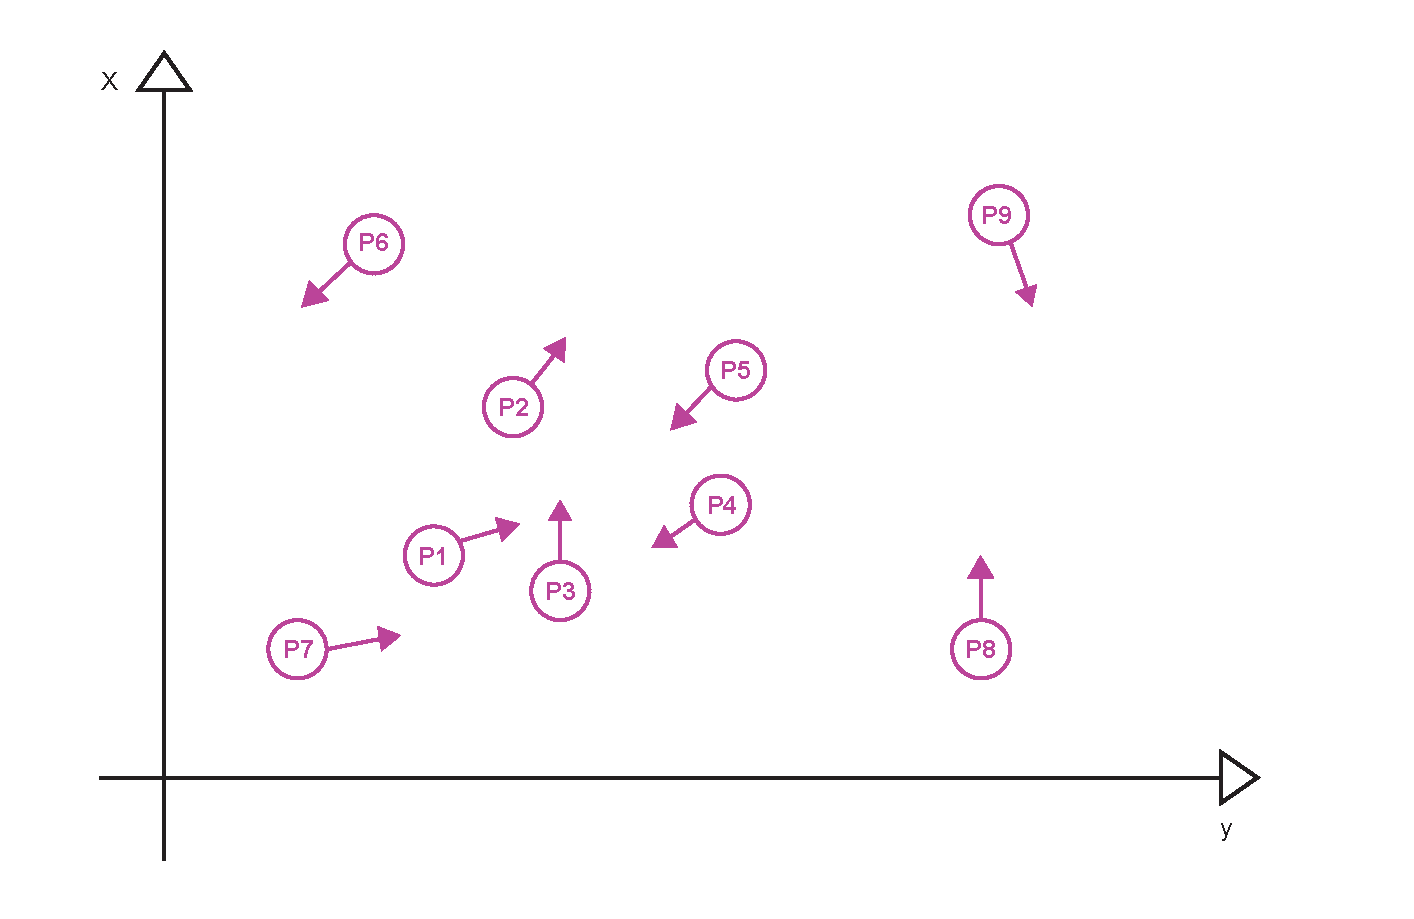
\includegraphics[width=4in]{assets/pso_diagram1.pdf}
  \caption{Illustration of particles in a 2D-space in an early iteration of the PSO algorithm (exploring)}
   \label{fig:psoBeginning}
\end{figure}

\begin{figure}[H]
  \centering
  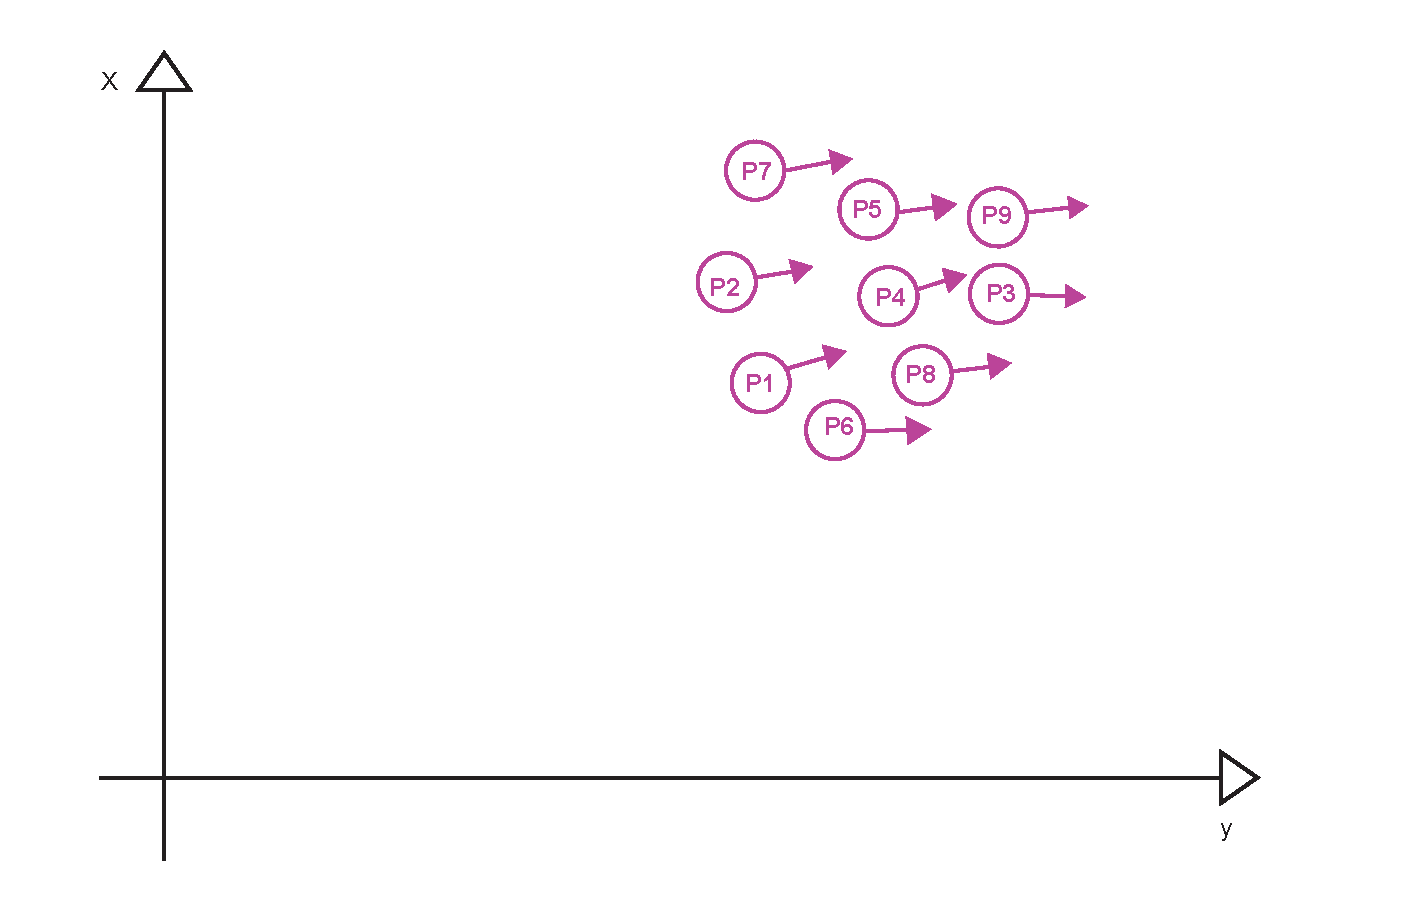
\includegraphics[width=4in]{assets/pso_diagram2.pdf}
  \caption{Illustration of particles in a 2D-space in a late iteration of the PSO algorithm (exploiting)}
   \label{fig:psoEnd}
\end{figure}




